\chapter{Передовые инструменты и технологии Андроид разработки}

Разработка мобильных приложений под Android непрерывно развивается. По мере того, как сообщество продолжает изучать новые способы разработки, Google продолжает предоставлять новые технологии, чтобы делать этот процесс еще проще и удобнее, развивая платформу и сообщество. 


\section{Высокоуровневый язык программирования Kotlin и библиотека Jetpack}

Kotlin -- это современный, статически типизированный, объектно-ориентированный, совместимый с Android язык программирования с открытым исходным кодом, который устраняет многие проблемы Java, такие, как исключения нулевого указателя или чрезмерная многословность кода. Kotlin был разработан профессионалами компании JetBrains. С 2019 года Google объявила Kotlin приоритетным языком программирования для разработки Android-приложений. Kotlin это безопасный, выразительный, лаконичный, универсальный и удобный для инструментов язык, который отлично взаимодействует с Java и JavaScript \cite{7}. Kotlin обладает выдающейся поддержкой современных IDE, таких, как Android Studio, IntelliJ Idea и Eclipse. Стандартные задачи, такие, как помощь с кодом или рефакторинг, выполняются правильно. 

В 2018 году Google представила сообществу разработчиков Android Jetpack -- набор программных компонентов, которые помогают в разработке выдающихся приложений для Android \cite{Kotlin4}. Эти программные компоненты помогают в решении следующих задач:
\begin{enumerate}
    \item соблюдение лучших практик;
    \item создание шаблонного кода;
    \item упрощение сложных вещей.
\end{enumerate}

Jetpack, разработанный для ускорения и упрощения разработки современных и надежных приложений для Android, состоит из набора инструментов, библиотек и рекомендаций по архитектуре \cite{8}. Jetpack помогает разработчикам писать код, который работает согласованно на всех версиях Android и на всех устройствах, чтобы разработчики могли сосредоточиться на коде.

\section{Coroutines легковесные потоки исполнения}

Coroutines -- это библиотека Kotlin для управления фоновыми задачами, такими как выполнение сетевых вызовов и доступ к файлам или базам данных, или выполнение длительных фоновых задач, а также является официальной рекомендацией Google для асинхронного программирования на Android \cite{book:Jomar}.

Официальная документация Kotlin квалифицирует Coroutines как «облегченные потоки», которые позволяют писать асинхронный неблокирующий код. Концепция вращается вокруг использования приостанавливаемых функций и точек приостановки \cite{kotlin5}.

Функция приостановки -- это функция, которая может выполнять свою задачу, приостанавливая поток, не блокируя его, поэтому поток все еще может выполнять другие задачи (рисунок \ref{fig:coroutine}). Когда функция приостановки будет выполнена, текущий поток возобновит выполнение. Это облегчает чтение, отладку и тестирование кода.

\begin{figure}[h!]
    \begin{center}
        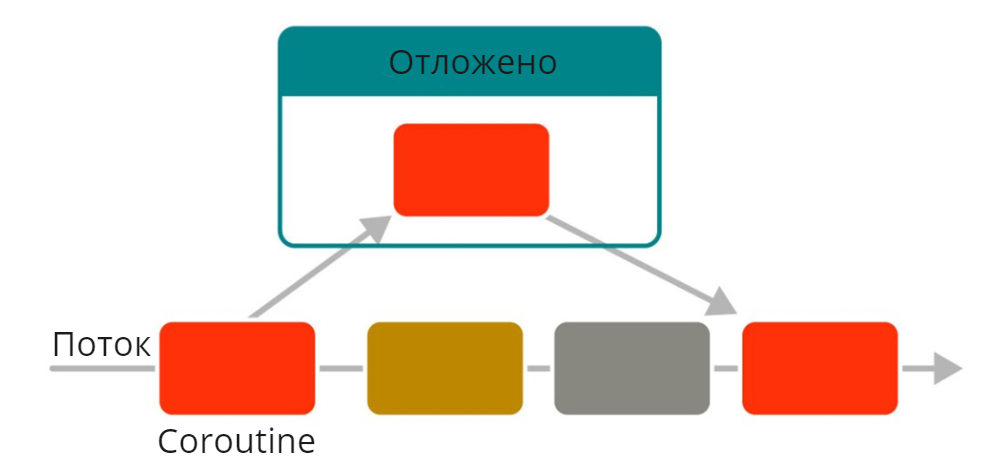
\includegraphics[width=0.95\hsize]{fig/coroutine.png}\\[2mm]
        \caption{Схема работы функции приостановки}\label{fig:coroutine}
    \end{center}
\end{figure}

CoroutineScope управляет жизненным циклом Coroutines в пределах четко определенной области или жизненного цикла. Это объект, который играет роль родителя в структурированном параллелизме, его цель -- управлять и отслеживать Coroutines, которые вы создаете внутри него.

Слишком много потоков может занимать много памяти, что в конечном итоге приведет к сбою программы. Coroutines не всегда создают новые потоки, они могут повторно использовать существующие из пулов потоков.

\section{Flow ассинхронный поток данных в Kotlin}

Flow - это библиотека асинхронных потоков Kotlin, построенная поверх Coroutines. Flow может выдавать несколько значений вместо одного значения и в течение определенного периода времени. Kotlin Flow идеально подходит для использования, когда нужно возвращать несколько значений асинхронно, например, при автоматическом обновлении из источника данных \cite{book:flow}. Flow интегрирован во многие библиотеки Jetpack и пользуется популярностью среди сторонних библиотек Android. 

Flow позволяет реализовать шаблон observer: шаблон проектирования программного обеспечения, состоящий из объекта, который поддерживает список своих зависимых элементов и автоматически уведомляет их о любых изменениях состояния (рисунок \ref{fig:flow}). 

Flow состоит из трех объектов:
\begin{enumerate}
    \item производитель. Создает данные, которые добавляются в поток;
    \item посредник. Может изменять каждое значение, передаваемое в поток, или сам поток;
    \item потребитель. Использует значения из потока.
\end{enumerate}

\begin{figure}[h!]
    \begin{center}
        
\includegraphics[width=0.95\hsize]{fig/flow.png}\\[2mm]
        \caption{Сущности, участвующие в потоке данных}\label{fig:flow}
    \end{center}
\end{figure}

В зависимости от типа наблюдателя потоки данных могут быть либо холодными, либо горячими. К холодным потокам относится Flow по умолчанию -- у потока нет состояния, код производителя выполняется каждый раз, когда в потоке выхывается оператором. К горячим же относят потоки типов StateFlow и SharedFlow, они позволяют потокам оптимально передавать обновления состояния и значения нескольким потребителям, такой тип потока никогда не завершается, он существует независимо от потребителей \cite{book:shrdflow}.

SharedFlow распределяет излучаемые значения между всеми своими потребителями широковещательным способом, так что каждый получают все излучаемые значения. Холодный поток можно преобразовать в горячий используя оператор \verb|shareIn|.

StateFlow оптимизированный подкласс SharedFlow, который представляет состояние, доступное только для чтения, с единственным обновляемым значением данных, которое отправляет обновления значения своим потребителям.





\section{Jetpack Compose новый инструмент UI}

Исторически иерархия Android View была представлена в виде дерева виджетов (рисунок \ref{fig:ViewHierarchy}) пользовательского интерфейса (UI). Все, что вам нужно было сделать, это определить пользовательский интерфейс в XML-файле и подключить его к вашему экрану (Activity) \cite{Kotlin2}. Это работало безупречно, потому что приложения были небольшими, и разработчикам нужно было поддерживать всего несколько устройств.

\begin{figure}[h!]
    \begin{center}
        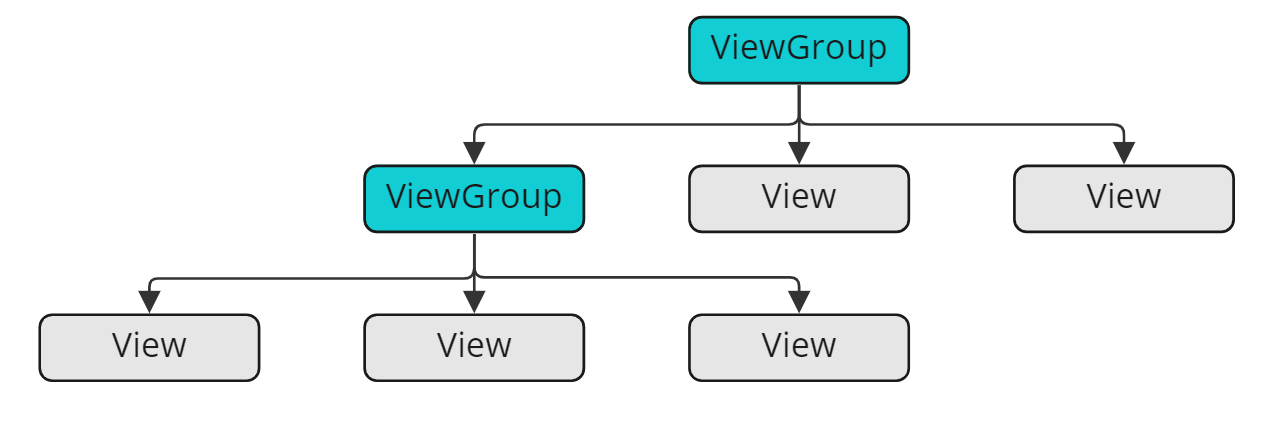
\includegraphics[width=1.05\hsize]{fig/view.png}\\[2mm]
        \caption{Иерархия View}\label{fig:ViewHierarchy}
    \end{center}
\end{figure}

Но сложность приложений значительно возросла; для выполнения базовых задач, таких как реализация списков прокрутки или анимации, требуется много шаблонного кода.

LayoutInflater — специальный компонент, который считывает определение XML и создает объекты Kotlin и Java (рисунок \ref{fig:NonScalableLayoutSystem}). Во время выполнения он раздувается до дерева компонентов \cite{Jetpack}.

\begin{figure}[h!]
    \begin{center}
        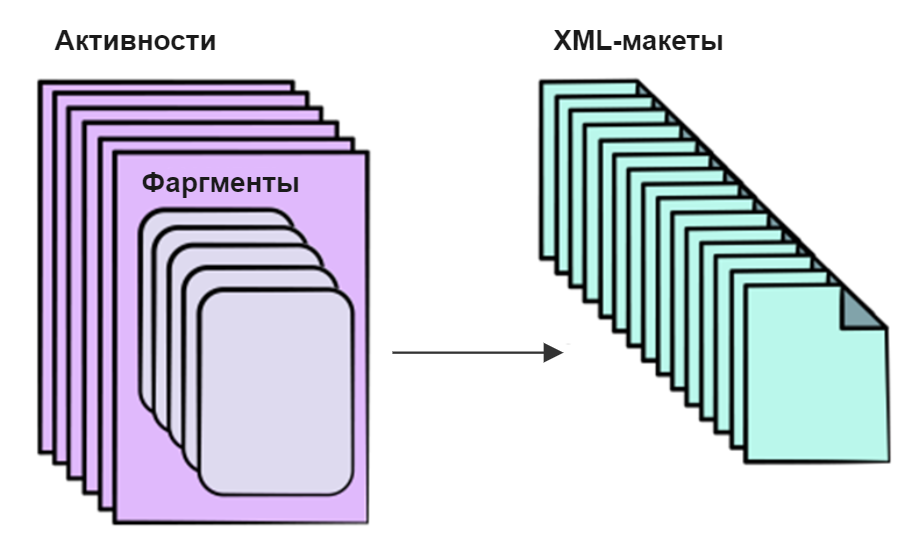
\includegraphics[width=0.85\hsize]{fig/nonxml.png}\\[2mm]
        \caption{Немасштабируемая система Layout}\label{fig:NonScalableLayoutSystem}
    \end{center}
\end{figure}

Чтобы изменить пользовательский интерфейс, необходимо изменить атрибуты всех связанных компонентов \cite{book:Xml1}. Даже если элемент пользовательского интерфейса не виден, он остается частью дерева компонентов \cite{Kotlin3}. Чем больше элементов пользовательского интерфейса в приложении, тем сложнее отслеживать такие изменения.

Jetpack Compose -- это современный инструментарий пользовательского интерфейса, предназначенный для упрощения разработки UI в Android, полностью построен на Kotlin. Он полностью декларативный, так что вы можете описать свой пользовательский интерфейс, вызвав некоторую серию функций, которые преобразуют ваши данные в иерархию пользовательского интерфейса (рисунок \ref{fig:UIAsDataFunction}). Когда данные изменяются или обновляются, фреймворк автоматически вызывает эти функции и обновляет представления.

\begin{figure}[h!]
    \begin{center}
        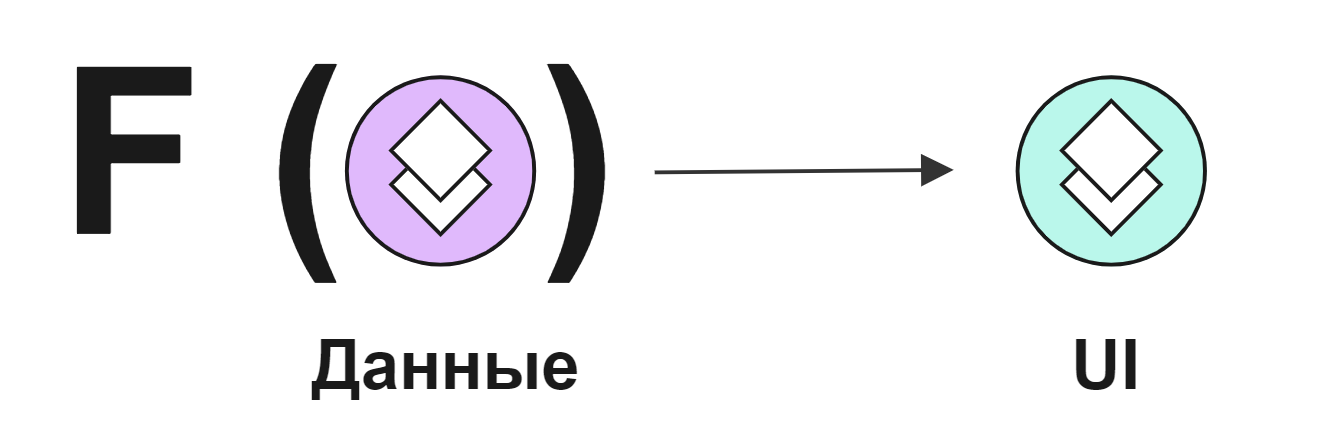
\includegraphics[width=0.85\hsize]{fig/fui.png}\\[2mm]
        \caption{UI как функция данных}\label{fig:UIAsDataFunction}
    \end{center}
\end{figure}

Наличие пользовательского интерфейса и бизнес-логики, написанных на одном языке, позволяет реорганизовать эти зависимости, чтобы уменьшить связность и повысить согласованность вашего кода.

\section{Room работа с локальной базой данных}

Room -- это ORM, библиотека объектно-реляционных сопоставлений.  Другими словами, Room сопоставит объекты базы данных с объектами Kotlin. Room предоставляет уровень абстракции поверх SQLite, позволяющий беспрепятственно получать доступ к базе данных, используя при этом все возможности SQLite \cite{book:ROOM}.

Room состоит из трех основных компонентов:
\begin{enumerate}
    \item entity. Представляет таблицу в базе данных. Room создает таблицу для каждого класса с аннотацией \verb|@Entity|, поля в классе соответствуют столбцам в таблице. Поэтому классы сущностей, как правило, представляют собой небольшие классы моделей, которые не содержат никакой логики;
    \item dao. Отвечают за определение методов, которые обращаются к базе данных. В исходном SQLite мы используем объекты \verb|Cursor| \cite{book:sqlite2}. С Room нам не нужен весь код, связанный с курсором, и мы можем просто определять наши запросы, используя аннотации в классе \verb|@Dao|;
    \item database. Содержит владельца базы данных и служит основной точкой доступа для базового подключения к сохраняемым реляционным данным вашего приложения. Чтобы создать базу данных, нам нужно определить абстрактный класс, который расширяет базу данных. Этот класс аннотируется \verb|@Database|, перечисляет сущности, содержащиеся в базе данных, и DAO, которые обращаются к ним.
\end{enumerate}


\section{DataStore улучшенная система хранения данных}

DataStore - это библиотека Google для сохранения данных в виде пар ключ-значение или типизированных объектов с использованием протокола буферов. Используя Kotlin Coroutines и Flow в качестве своей основы, он стремится заменить SharedPreferences. Поскольку он является частью набора библиотек Jetpack, он также известен как DataStore Jetpack \cite{book:dataStore}.

DataStore предлагает две реализации, из которых вы можете выбрать одну в зависимости от варианта использования:

\begin{enumerate}
    \item preferences DataStore. Хранит данные в виде пар ключ-значение, аналогично SharedPreferences. Используется это для хранения и извлечения примитивных типов данных;
    \item proto DataStore. Использует протокол буферов для хранения пользовательских типов данных. При использовании Proto DataStore вам необходимо определить схему для пользовательского типа данных.
\end{enumerate}

SharedPreferences использует XML для хранения данных. По мере увеличения объема данных размер файла резко увеличивается, и процессору обходится дороже читать файл.

Протокол буферов - это новый способ представления структурированных данных, который работает быстрее, чем XML, и имеет меньший размер. Они полезны, когда время чтения сохраненных данных влияет на производительность вашего приложения. Чтобы использовать их, вы определяете свою схему данных с помощью файла .proto. Затем зависящий от языка плагин генерирует для вас класс.

DataStore обеспечивает возможность асинхронного доступа к данным, что позволяет избежать блокировки основного потока приложения.

\section{Внедрение зависимостей в Android приложении}

Внедрение зависимостей (DI) -- это метод, широко используемый в программировании и хорошо подходящий для разработки Android, где зависимости предоставляются классу вместо того, чтобы создавать их самому. На рисунке \ref{fig:DI} приведено сравнение традиционных компонентов и DI-компонентов.

\begin{figure}[h!]
    \begin{center}
        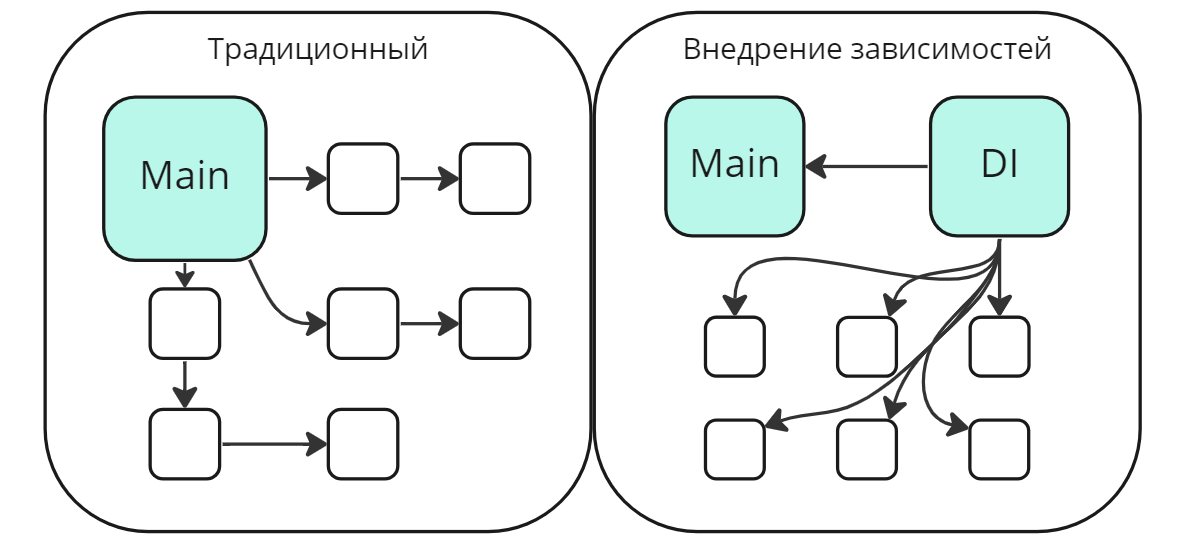
\includegraphics[width=0.95\hsize]{fig/di.png}\\[2mm]
        \caption{Сравнение традиционных компонентов и DI-компонентов}\label{fig:DI}
    \end{center}
\end{figure}

Внедрение зависимостей (DI) -- это шаблон проектирования, используемый для реализации инверсии управления (IoC), что означает, что поток приложения инвертируется. Мы можем создать зависимый объект вне класса и предоставить эти объекты классу различными способами. DI может помочь с переносом создания и привязки зависимых объектов за пределы класса, который зависит от них.

При написании приложений программисты сталкиваются с проблемой написания большого количества шаблонного кода, например фабрик.

Использование внедрения зависимостей предоставляет следующие преимущества:

\begin{enumerate}
    \item возможность повторного использования кода;
    \item простота рефакторинга;
    \item простота тестирования.
\end{enumerate}

Фреймворки внедрения зависимостей -- это специальные библиотеки, которые помогают вам внедрять внедрение зависимостей в ваши проекты. Разные фреймворки предлагают разные шаблоны и разные утилиты, а также предполагают разные архитектурные и операционные компромиссы. Популярные фреймворки для внедрения зависимостей Android:

\begin{enumerate}
    \item dagger. Это легкий фреймворк с открытым исходным кодом от Google. Использует обработку аннотаций для генерации кода, высоко оптимизирован для приложений Android, позволяет разработчикам легко настраивать сгенерированный код, что делает его очень мощным;
    \item koin. Это библиотека с открытым исходным кодом, полностью написанная на Kotlin, предоставляет другой способ внедрения зависимостей -- использует модули, в которых объявляются все классы или фабрики, которые будут внедрены в качестве зависимостей в другие классы;
    \item hilt. Это фреймворк для внедрения зависимостей, построенный поверх Dagger. Предоставляет собой набор компонентов и аннотаций, которые упрощают настройку Dagger, а также рекомендации по структурированию кода. Разработан как более удобный вариант для начинающих.
\end{enumerate}